\section{Rough sketch of the cobordism hypothesis and extended topological field theories \extra}\label{sub:outlook_on_the_cobordism_hypothesis_and_extended_topological_field_theories}
 Recall that a TFT is
 \begin{itemize}
\item a way to organize invariants of smooth manifolds and compute them
\item a way to make (some) quantum field theories mathematically rigorous
 \end{itemize} 
 From the point of view of mathematics one might ask if we classify TFTs as we did for dimension 1 and 2 for any dimension $n$. From the point of view of physics one might ask if a TFT describing a certain physical system can be determined by the behavior of the system around a point, i.e. if it is fully local. The answer to these questions is yes and is called the cobordism hypothesis.

\begin{rem}[What is the cobordism hypothesis?]\label{RemarkOnCobHypo}
 The cobordism hypothesis informally states that any TFT, at any dimension, can be classified/constructed just by observing where the TFT in question sends the point\footnote{We will soon see a proof of the 1-dimensional case \ref{ClassificationOf1dTFTs}.}, i.e. a bit more rigorously
    \begin{thm}[Cobordism hypothesis]
        Let $\cat$ be a monoidal $(\infty,n)$-category with duals\footnote{We later give a definition of $(\infty,n)$-category with duals, see \ref{HigherMonCatDuals}.}. Then the evaluation functor on a point, i.e. the functor sending $\Zf\mapsto \Zf(\ast)$, induces an equivalence 
        $$ev_{\ast}:\Fun^{\otimes}(\Bord_{n},\cat)\to (\cat^{\operatorname{fd}})^{\cong}$$
        where $\cat^{\operatorname{fd}}$ is the full\footnote{i.e. there are all morphisms between the objects of the subcategory, i.e. no morphism from the category is forgotten.} monoidal $(\infty,n)$-category with duals\footnote{We gave a definition of $(\infty,n)$-category with duals, see \ref{HigherMonCatDuals}.}, i.e. we
         forget about all non-dualizable objects, and $\cat^{\cong}$ is the maximal underlying groupoid of $\cat$, i.e. we
          forget about all morphisms that are not invertible.
    \end{thm}
    It was formulated by James Dolan and John Baez in \cite{Baez_1995} and now we have only partial proofs,
     \cite{lurie2009classification}, \cite{ayala2017cobordism} and \cite{grady2022geometric}. The one by Ayala and
      Francis relies has a different strategy to the first sketch by Lurie and relies on an unproved conjecture regarding
       factorization homology, see \ref{FactorHomology} for a definition of factorization homology.
    \end{rem}
\begin{rem}[What are extended TFTs?]\label{RemarkExtendedTFTs}
    After defining the cobordism hypothesis in this manner, a natural question is: how can TFTs of any dimension greater than 1 be classified by evaluating them at a point? If we stick to our definition, there are no points in any category of bordisms of dimension greater than 1. Fortunately, one can \emph{extend} the bordism category, and consequently TFTs, and also talk about lower dimensions. Take as an example $\Bord^{or}_{2,1}$. As we defined the bordism category, in this case the lowest dimension is 1, the objects are lines, not points. Nevertheless, one could treat the category of 2 dimensional bordisms as a 2-category, more specifically as a bicategory (see \ref{Bicategory})\footnote{Since 1-morphisms do not compose strictly, but up to an appropriate notion of isomorphism.}, $\Bord_{2,1,0}$ where objects are disjoint unions of points, 1-morphisms are oriented cobordisms between points and 2-morphisms are cobordisms between the 1-morphisms; and then define 2d-TFTs as an
     appropriate notion of symmetric monoidal functor between symmetric monoidal bicategories\footnote{A detailed
         treatment of the 2d case is found in \cite{schommerpries2014classification}.} (see \ref{SymmMonBicategory} for a definition).  
         However, to this we need to allow manifolds with corners, as the illustration of the downward extension of the torus shows (\ref{CUTTORUS}).
    \begin{figure}
        \centering
        \captionsetup{format = hang}
        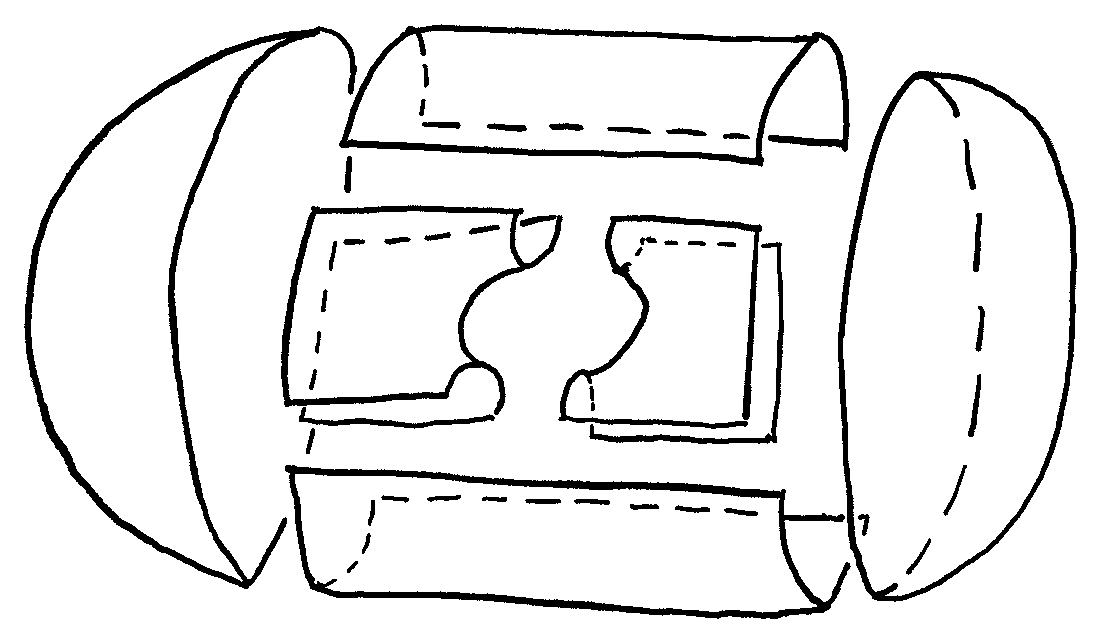
\includegraphics[width=9cm]{images/Final Lecture/TorusExtendedCut.png} 
        \caption{\small{Visualization of a torus extended down to a point. The vertices of the corners of the 2-dimensional surfaces are points.}}
        \label{CUTTORUS}
    \end{figure}
    
    Treating a TFT as a symmetric monoidal weak 2-functor (see \ref{Weak2Fun} for a definition)
     from
     a symmetric monoidal bicategory 
    $\Bord_{n,n-1,n-2}$
    (see \ref{SymmMonBicategory} for a definition), instead of from a symmetric monoidal category
     is
     named 'once-extended TFT', e.g. see \cite{SchwHopfQuantumTFT}. There are two important
      results
      regarding once-extended TFTs: 
    \begin{enumerate}
\item One regards the classification of 2d-TFTs down to a point and is due to Christopher Schommer Pries who
 proved it in his PhD thesis 
 $$
 ev_{\ast}:
 \Fun^\otimes (\Bord_{2,1,0}^{\fr}, \bat) \xrightarrow{\simeq} (\bat^{2\operatorname{-dualizable}})^{\cong} $$
\item The other, although still conjectural\footnote{It was first stated by Kevin Walker and then some progress was made by Turaev, see \cite{Turaev+2016} for more on this.}, classifies 3d-TFTs via the evaluation on the circle
$$  ev_{S^1}:\Fun^\otimes (\Bord_{3,2,1}^{\fr}, \operatorname{ModTensor}) \xrightarrow{\simeq}(\operatorname{ModTensor}^{2\operatorname{-dualizable}})^{\cong}$$ %unsure about the statement, did not find clearr references /ANdrea
hence $\Zf(S^1)=\cat$ where $\cat$ is a modular tensor category, i.e. a special ribbon category which can be seen as a categorified commutative Frobenius algebra.
    \end{enumerate}
    
    However, as one can infer from the aforementioned cobordism hypothesis, one can also extend downward to dimension $0$ any $n$-dimensional TFT and it was first proposed by Daniel Freed in \cite{Freed_1994}. To be precise, one nowadays does not want to only extend 
    downwards but also upwards, i.e. to not work wirh $n$-categories, i.e. $(n,n)$-categories,
     but wants to work with$(\infty,n)$-categories, i.e. categories where morphisms of dimension
      strictly greater than $n$ are invertible, because of technical reasons\footnote{For example, the
         argument sketched in \cite{lurie2009classification} is crucially a proof by induction on $n$
          and in order to understand the $n+1$-morphisms of $\Bord_{n+1}$ one must understand
           such $n+1$-morphisms in $\Bord_{n}$ which are absent if we treat $\Bord_{n}$ as an
            $n$-category and not $(\infty,n)$-category. In short, that would just not be possible
             without such $\infty$-categorical machinery.}. 
     Sketchily, the $(\infty,n)$ category of bordisms will have points as objects, bordisms between
      points as 1-morphisms, bordisms between bordisms between points as 2-morphisms,...,
       bordisms between bordisms between bordisms...\footnote{There is exactly $n-1$ times
         'between bordisms' after the first instance of 'bordisms', $n$-morphisms are morphisms
          between $(n-1)$-morphisms.} as $n$-morphisms, diffeomorphisms between
           $n$-dimensional bordisms as $n+1$-morphisms, isotopies between diffeomorphisms as
            $n+2$-morphisms, isotopies between isotopies between diffeomorphsims as
             $n+3$-morphisms, ... and so on infinitely many times.
              This is an example of a $(\infty,n)$-category, since isotopies of diffeomorphisms and
               diffeomorphisms are in fact invertible, whereas oriented bordisms not necessarily.
                One can find more on this higher category of bordisms in \cite{Calaque_2019}. 

\end{rem}